\documentclass[fleqn,10pt]{wlscirep}
\usepackage[utf8]{inputenc}
\usepackage[T1]{fontenc}
\usepackage{comment}
\usepackage{svg}
\usepackage[backend=biber,natbib,style=apa,autocite=inline]{biblatex}
\usepackage{lineno}
\fancyhead[LO]{\textit{Reshaped functional connectivity gradients in acute ischemic stroke}}
\usepackage{color}
\usepackage{soul}
\linenumbers
\addbibresource{sample.bib}
\bibliography{sample.bib}
\title{Reshaped functional connectivity gradients in acute ischemic stroke}

\author[1,*]{Cemal Koba}
\author[1]{Joan Falc\'o-Roget}
\author[1,2]{Alessandro Crimi}
\affil[1]{Sano Centre for Computational Medicine, Czarnowiejska 36, Krak\'ow, 30-054, Poland}
\affil[2]{Faculty of Computer Science, AGH University of Krakow Mickiewicza 30, Krak\'ow, 30-059, Poland}
\affil[*]{Correspondence: c.koba@sanoscience.org}




\begin{abstract}
Ischemic brain stroke disrupts blood flow, leading to functional and structural changes associated with behavioral deficits. Importantly, despite this disruption occurring in localized regions, the resulting changes in the functional organization are both high-dimensional and widespread across the human cortex. However, the mechanisms with which these global patterns emerge and the subsequent behavioral deficits they entail, remain largely unexplored. Functional connectivity gradients provide consistent, reproducible, and robust low-dimensional representations of brain function that can be explored to reduce brain heterogeneity to a handful of axes along which brain function is organized. Here, we investigated how stroke disrupts this canonical gradient space by aligning each patient to a control-averaged gradient embedding and computing the distances to the "correct" positions to quantify functional deviations and their contribution to behavioral deficits. Importantly, we explicitly corrected these gradients for stroke-induced hemodynamic lags to further study their contribution. We found that lag correction enhanced the functional connectivity gradients most prominently in the second gradient, on which visual and somatomotor function is concentrated. Additionally, we identified significant functional deviations primarily within somatomotor, visual, and ventral attention networks, correlating with behavioral impairments. We studied the hemispheric asymmetries of these deviations finding that intact hemispheres preserve comparable patterns of asymmetry while damaged ones presented important changes. Lastly, right-sided lesions displayed more localized functional deviations than their contralateral lesions. Overall, we provide evidence that 1) correcting for hemodynamic lags improves gradient accuracy, as indicated by increased percentages of explained variance, and 2) behavioral impairments and hemispheric asymmetries result from a repositioning of region-based connectivity profiles in a low-dimensional, interpretable space. This suggests that large-scale brain function alterations manifest in slight, predictable movements largely confined to the visual-somatomotor axis.

%This study investigates the impact of acute ischemic stroke on brain functional organization and evaluates the influence of temporal lag correction on connectivity gradients. We employ dimensionality reduction techniques to represent complex neural functions across three orthogonal gradients, offering a macroscopic view of brain function alterations due to stroke. In addition, we account for the temporal lag aberrancies that are prevalent in stroke-affected regions due to the disrupted blood flow. We identified significant functional deviations primarily within somatomotor, visual, and ventral attention networks, correlating with behavioral impairments. Additionally, we observed negative correlations between functional deviation and left motor, spatial memory, and visual bias performance. Temporal lag correction significantly alters gradient values, particularly along the superior-inferior axis, enhancing alignment with the temporal domain. Stroke subjects benefit notably from this correction, with pronounced differences observed in the visual-somatomotor gradient.



\end{abstract}


\begin{comment}
    Ischemic stroke leads to aberrant neural dynamics and metabolic changes, causing various behavioral and neural dysfunctions. This study investigates the impact of ischemic stroke on macroscale functional organization using functional connectivity gradients.

Altered connectivity patterns asischemic stroke, and dimension reduction techniques provide a holistic perspective. However, the temporal characteristics of the blood oxygen level-dependent (BOLD) signal, influenced by stroke-induced time delays, present a challenge in accurately assessing functional connectivity. This paper explores the effects of ischemic stroke on macroscale functional organization and evaluates the influence of temporal lag correction on functional connectivity gradients.
The study utilizes a three-dimensional metric derived from connectivity gradients to characterize the deviations in functional organization caused by stroke. Hemispheric differences in acute ischemic stroke are expected based on previous findings, and the correction for time lags is anticipated to enhance functional connectivity gradients, particularly for stroke patients. After correction, the residual differences are hypothesized to primarily reflect functional disparities rather than metabolic variations.
The results contribute to a comprehensive understanding of the consequences of ischemic stroke on the brain's functional architecture, shedding light on the potential relationships between structural, and behavioral measures, and connectivity deviations. Furthermore, this research emphasizes the importance of temporal lag correction in improving the accuracy of functional connectivity analysis, not only in stroke patients but also in healthy controls. The findings have implications for advancing our understanding of stroke-related alterations in brain function and may inform future interventions for stroke patients.
\end{comment}

\begin{document}

\flushbottom
\maketitle
% * <john.hammersley@gmail.com> 2015-02-09T12:07:31.197Z:
%
%  Click the title above to edit the author information and abstract
%
 \textit{Keywords: Stroke, fMRI, gradients, temporal lag, BOLD}

\textcolor{blue}{Revised version after 1st round of revisions from  NI: Clinical}
\section*{Introduction} 
Ischemic stroke occurs when a vessel supplying blood to the brain is obstructed, ultimately leading to blood shortage \citep{Roach_Bettermann_Biller_2010}, causing abnormal neural dynamics even if the blockage is short in time. Importantly, if the impairment lasts long enough, neural death is unavoidable. The infarcted region directly suffering from lack of blood will likely be surrounded by swelling \citep{hong2021hemorrhagic}, thus extending the structural damage to areas near the onset region. Moreover, large population studies have shown that these infarcted regions are not randomly distributed across the brain, but rather subcortical areas are more likely to be affected \citep{thiebaut2020brain,weaver2019meta}. Even though a significant heterogeneity concerning the exact location of the ischemia exists, the basal-ganglia networks, the cerebellum, and the cerebrospinal tracts are commonly affected brain areas. Consequently, given the emerging role of such structures in the coordination of distributed and localized neurological functions \citep{bostan2013cerebellar,quartarone2020new}, the diverse findings from functional magnetic resonance imaging (fMRI) studies become more comprehensible. 

FMRI crucially relies on the association between the metabolic consumption that neural activity incurs. However, if blood flow is impaired, there is no guarantee that the blood oxygen level-dependent (BOLD) signal reflects artifacts stemming from the stroke or the underlying activity of neural tissue. Crucially, the signal within lesioned areas has been shown to be temporally delayed \citep{siegel2016effects}, showing peaks at later time values \citep{altamura2009longitudinal,bonakdarpour2015variability}. Furthermore, stroke patients also displayed power spectra that were shifted towards lower frequencies, thus having slower oscillations \citep{siegel2016effects}. This empirical delay can be exploited to create perfusion maps solely from the fMRI series \citep{lv2013identifying,tong2017perfusion,khalil2020non,braban2023cerebrovascular} by applying temporal shifts so that the cross-correlation between the voxel-wise and a reference signals (e.g., global signal, venous sinuses) is maximum. This \textit{time-lag correction} highlights areas with delayed blood flow, improves the data-quality \citep{erdougan2016correcting}, and enhances the functional connectivity in control groups \citep{tong2017perfusion} while maintaining the relationships with behavioral dysfunctions in stroke studies \citep{siegel2016effects}. Importantly, the altered functional topographies of patients are thought to arise from impaired neural function rather than exogenous blood shortage. Nonetheless, time-lag corrections are not ubiquitously practiced \citep{bayrak2019impact}, thus adding another layer of heterogeneity to the analyses.

Amongst the wide range of observed behavioral deficits in stroke populations, motor, linguistic, and attention-related are the most common ones \citep{he2007breakdown}. For example, during arm-moving tasks, the contralesional hemisphere shows a hyper-activity that, in turn, reduces to baseline levels with the recovery-time \citep{rehme2011role}. Moreover, the degree of this imbalance between ipsi and contralesional hemispheres after post-stroke is descriptive of motor recovery \citep{dodd2017role}. Resting-state (RS) studies broadly converge to a decrease in inter-hemispheric connectivity (i.e., lower Pearson correlations between fMRI series), an increase in connectivity within the contralesional hemisphere \citep{new2015altered,yourganov2021effect}, and an abnormal functional co-activation between intact and damaged hemispheres \citep{carter2010resting}. In general, altered homotopic connectivity predicts lesion size and severity \citep{urbin2014resting,tang2016decreased}, while specific behavioral deficits are related to damaged connectivity in the corresponding RS network \citep{corbetta2002control,carter2010resting}. But functional data is high-dimensional therefore compromising inferences. Network studies reduce the size of the system by introducing an additional layer of abstraction, where macroscopic regions are used instead of voxels \citep{Schaefer_2017}. Although the hub structure of such networks is significantly damaged in stroke patients \citep{gratton2012focal,zhu2017disrupted}, the resulting clinical correlates remain unclear. In addition, intra-class correlation scores are rather low for voxel- and region-wise studies \citep{noble2021guide}. Considering these drawbacks for clinical applicability, explicit dimensionality reduction techniques may help to understand the consequences of stroke from a more general point of view. In this regard, functional connectivity gradients \citep{margulies2016situating} display the macroscale functional organization instead of discrete and specific connectivity characteristics between regions or network-based statistics. 

Gradients of brain function project the complex functional profiles along three orthogonal axes encapsulating most of their variance \citep{vos2020brainspace}. Importantly, they have been proven to be highly replicable \citep{margulies2016situating,bethlehem2020dispersion,mckeown2020relationship,hardikar2022macro}. In healthy cohorts, the major axis splits the cortex into unimodal and multimodal areas, the second axis separates visual and somatomotor functions, and the third gradient distinguishes active-passive attention modalities \citep{Glasser_2016}. But, in clinical groups, slight deformations of these axes were found to be descriptive of specific syndromes, such as autism \citep{hong2019atypical} and depression \citep{xia2022connectome}. In stroke, only one study considered this framework to understand the macroscale organization of the brain (dys-)function \citep{bayrak2019impact}. Gradient coordinates of voxels within the lesioned sites from the healthy cohort were compared to intact voxels from patients. This yielded a functional distance map that was proportional to the stability of the functional profile over recovery time. Simplifying, voxels that were far from the lesion, in terms of functional similarity, remained largely unaltered through time. However, the data was not corrected for time-lag aberrancies, and masking of the infarcted areas was based on human annotations thus considering the lesion only in an indirect way (i.e., the lesioned signal was discarded). Moreover, these conclusions solely applied to the 1st and 3rd gradients, leaving the visual and somatomotor axis unstudied. 

In this 3-dimensional space, each voxel or region of interest (ROI) is uniquely determined by 3 spatial coordinates which, after a correct alignment preserving the original distances between points \citep{vos2020brainspace}, can be taken as the canonical position in health. We hypothesize that 1) lag-correction repositions each region and increases the alignment with respect to the canonical locations, especially in patients suffering from ischemic stroke, and 2) the position in this space is indicative of functional and behavioral impairments. Although, several metrics have been derived for this purpose \citep{del2022higher,valk2023functional}, we opt for an interpretable distance function between any two points in space (i.e., euclidean distance between healthy controls and stroke subjects), which we aim to be predictive of behavioral and clinical correlates. We also describe several other known phenomena related to hemispheric differences that affect the functional connectivity gradients.
\begin{comment}
  
-------------- OLD VERSION ---------------

\color{green}Ischemic stroke occurs when a vessel supplying blood to the brain is obstructed, ultimately leading to blood shortage \citep{Roach_Bettermann_Biller_2010}. Lack of blood flow, even for a short time, causes abnormal neural dynamics. If it lasts long enough, neural death is unavoidable. The region that suffers from the lack of blood flow will be infarcted, and there is a chance that the surrounding region will be swollen \citep{hong2021hemorrhagic}. These changes in the brain's structure are associated with a wide range of behavioral and neural dysfunctions, not only within the lesion site but also in its anatomically and functionally connected areas. Motor, linguistic, and attention-related behavioral deficits are commonly observed in stroke patients \citep{he2007breakdown, siegel2016disruptions}. Task and resting-state (RS) activity and networks that are related to those functions are therefore subject to change. During arm-moving tasks, the contralateral hemisphere shows over-activity \citep{rehme2011role}. This over-activity decreases with the recovery time. RS studies showed that the behavioral deficits are related to the decrease in the connectivity of their respective pre-defined network (e.g. motor dysfunction and motor network - \cite{carter2010resting}, attention performance with attention network - \cite{corbetta2002control}). The decreases show the difference between intact and damaged hemispheres \citep{carter2010resting}. In general, decreased overall connectivity between hemispheres, and increased overall connectivity within the contralateral hemispheres to lesions are observed \citep{new2015altered, yourganov2021effect}. This difference in lateralization is also reported via homotopic connectivity. Decreased connectivity between homotopic regions of stroke subjects between intact and damaged hemispheres has been related to the lesion size and severity \citep{urbin2014resting, tang2016decreased}. Lastly, the network-based approach is also a useful method for reporting stroke-related differences. Altered nodal degrees in the default mode network were found for stroke patients \citep{zhu2017disrupted}. In addition, damage to connector hubs seems to make the most of the connectivity difference \citep{gratton2012focal}. \color{black}


The effect of stroke on brain function and structure varies depending on the extent and the location of the lesion, making it difficult to make group-level inferences on pre-defined resting-state (RS) networks. \color{green}However, studies with large sample sizes show that the occurrence of the ischemic stroke is not random \citep{weaver2019meta, thiebaut2020brain}. The most common regions that are affected by ischemic stroke are basal ganglia, cerebrospinal tract, and cerebellum. Considering this dichotomy of the individual and sample characteristics, dimension reduction techniques, such as functional connectivity gradients \citep{margulies2016situating, vos2020brainspace} may help in understanding the consequences of stroke from a more general point of view, as it displays the macroscale functional organization, rather than discrete and specific characteristics of the connectivity such as functional connectivity of regions or network-based statistics. The connectivity gradients approach shows the major axes of the brain's functional organization. The most dominant axis is organized from unimodal to transmodal functions, meaning that brain function can be explained mainly by these two sides of the same gradient. Following the first one, the second gradient indicates somatomotor-visual functions, and the third gradient shows active-passive attention. The gradients of brain function are highly replicable \citep{margulies2016situating, hardikar2022macro, mckeown2020relationship, hong2019atypical, bethlehem2020dispersion}.

Differences in gradient scores (indicating a region's position on the functional gradient) proved to show meaningful differences in the functional organization of clinical groups (autism - \cite{hong2019atypical}, depression - \cite{xia2022connectome}). \color{red} Further metrics that can be derived from the gradients are related to the 3D distribution of the functional organization, such as gradient range and variation \citep{del2022higher}, dispersion (distance of each node to the centroid of the network, \cite{valk2023functional}) and eccentricity (distance of each node to the centroid of the coordinate system \cite{valk2023functional}). \color{green} Among the studies that explore brain organization via connectivity gradients, only one study used stroke patients as the subject of interest \citep{bayrak2019impact}. The authors used "functional distance to lesion" as a metric, which is the similarity between the gradient score of any given point on the brain and the lesion area. They reported that this metric and functional connectivity stability over time are related. The closer a region is to the lesion on functional space, the more unstable it is. This relationship was reported for the 1st and the 3rd gradients.  

Apart from the heterogeneity of the stroke lesions at the individual level, another concerning issue for stroke research is the difference in the blood oxygen level-dependent (BOLD) signal from the lesioned areas. \color{red}By description is ischemic stroke, the BOLD signal, which is dependent on blood flow, shows different temporal characteristics compared to that of healthy tissue during both task and resting state fMRI. \color{green}To exemplify, the BOLD of stroke patients showed later peak values \citep{altamura2009longitudinal, bonakdarpour2015variability}, and are in a lower frequency domain  \citep{siegel2016effects}. Recent advancements in fMRI techniques showed that it is possible to detect stroke lesions via perfusion maps that are created solely from BOLD data. This technique calculates the time lag between a voxel and a reference time series (e.g. global signal - GS, or venous sinuses) \citep{tong2017perfusion, lv2013identifying,braban2023cerebrovascular,khalil2020non}. The lag maps highlight the areas with delayed blood flow, hence the lesioned areas. Correcting the RS data for these time lags increased the strength of the functional connectivity, assuming that the lesioned areas become more comparable with non-lesioned areas \citep{siegel2016effects}. The time lag is thought to be resourced from the lack of blood flow in the lesioned areas. However, even after correction, the relationship between behavioral dysfunction and functional connectivity metrics persists \citep{siegel2016effects}. When this method is applied to healthy subjects, a degree of improvement in the data quality is observed \citep{erdougan2016correcting}. This step aligns the data on the temporal domain, eliminating the temporal differences caused by the blood flow. In addition, \citet{tong2019low} discuss that delay maps also contain noise from very low-frequency oscillations such as cardiac and respiratory signals, therefore correcting for them improves the functional connectivity for the healthy controls.\color{black} 

In this study, the effect of ischemic stroke on the macroscale functional organization and the effect of temporal lag correction on the functional connectivity gradients are explored. Thanks to the 3D organization derived from the connectivity gradients, stroke subjects are expected to have larger deviations compared to control subjects. The deviations in 3D space are expected to be related to the structural and behavioral measures. Considering the previous reports on the hemispheric differences in the case of acute ischemic stroke, a hemispheric difference in the deviation is expected. Lastly, correction for the time lag is expected to improve the gradient distribution, more so for stroke patients. After the lag correction, the remaining difference is expected to reflect the difference due to function, rather than the difference in the metabolic differences. 
  
\end{comment}
\begin{comment}
    Resting-state (RS) BOLD reflects the temporal neural dynamics indirectly. However, metabolic blood flow can be also observed via the same data. \citet{mitra2014lag} It is important to distinguish if RS reflects the coherence due to the blood flow or neural dynamics. Temporal lag correction based on a reference time series (global signal - GS or venous sinuses) is a common method to examine the source of the BOLD signal. BOLD time series is time-shifted to the point that maximizes the correlation with the reference signal. It was shown that this correction increases the strength of the functional connectivity. The increased strength implies that the reference time series actually reflects the metabolical blood flow, and reordering the time series is a necessary preprocessing step like motion correction, slice-time correction etc... Most common reference signal is the GS, which is related to negative correlations across regions after correction. 

It is well-reported that GS correction of the RS data introduces negative correlations. It was shown that these negative correlations are related to the temporal order of the other BOLD series. GS reflects the mean BOLD activity and the metabolic flow. Therefore, voxels that are later in the metabolic order show negative correlations with the earlier ones after GS correction. Another study used venous sinuses, and they found similar results too. However, Removing GS after correcting for temporal lag was shown to eliminate the negative correlations caused by the metabolic blood flow and accounted for the mean neural activity only. However, the internal carotid artery (ICA) is the area that feeds the brain. Therefore, the reference signal should be BOLD activity from ICA. 


Temporal dynamics of the BOLD signal show the intracranial metabolic blood flow. Resting state networks also point out this order of blood flow up to some extent. It is important to differentiate this metabolic blood flow and blood flow due to the neural activity. 


It is possible to track the abnormalities in the blood flow in ischemic stroke cases via rs-FMRI. Temporal BOLD delay in reference to the GS reveals the infarcted regions. In line with the lag-correction studies of healthy subjects, blood supply is even more delayed in stroke-related regions. Therefore, lag correction would eliminate the negative correlations/associations sourced from delayed blood flow in stroke regions and reflect the neural differences more accurately. Delayed blood flow in the stroke-affected regions makes sense because ischemic stroke causes cessation of blood flow and ideally, BOLD signal from such areas should have zero variance as there is no activity. However, thanks to the collateral blood supply and recovery of the affected arteries, blood flow is still going on but slower/at a lower frequency than the regular cycle. 

Functional connectivity gradients reveal the structural-functional organization of the brain. In case of stroke, this organization may be altered. 

In this paper, we hypothesize that adjusting the BOLD signal from the infarcted regions in reference to the global signal will decrease the atrophy in the functional connectivity gradients between stroke patients and healthy controls.

\textcolor{blue}{Ideas for other papers or additions to this paper:
\begin{itemize}
    \item Check if the BOLD difference in stroke is due to time lags only or also due to slow oscillations
    \item Check if the lag difference can be better identified with ICA as the reference signal
    \item Check phase difference: What is the phase to build the successful gradient, and how this phase is different in stroke regions
    \item What is the extent of the neural changes in the "unaffected brain"? Create an unaffected brain map by accounting for the structural, functional, and arterial connectivity map of the stroke region.
    \item Longitudinal changes: how the brain recovers the gradients across across time. This can be calculated via Euclidian difference of each point in the embedding space. The dispersion will decrease over time.
    \item Use the lag-maps for automatic segmentation or predicting behavioral deficits using deep learning
    \item Hemispheric difference: extend the presentation for JU. 
    \item source of the time lag: arterial concentration, vessel diameter, flow time? 
\end{itemize}
}



The effect of stroke is unique across each participant because the location, extent, and recovery of the damage are unique to each patient. Therefore, investigating the effect of stroke at the group level would not show the real interaction/plasticity of the brain. If the goal of this line of research is to understand brain dynamics by observing the complications in the brain (like reverse engineering) and understanding their behavioral outcomes, every unique case must be examined individually. 

Ischemic stroke is a case of lack of blood flow to arteries in the brain. Lack of blood flow even for a short time causes abnormal neural dynamics and if it lasts long enough, neural death is unavoidable. The region that suffers from the lack of blood flow will be infarcted, and there is a chance that the surrounding region will be swollen. The change in the metabolism of the brain is associated with a wide range of behavioral dysfunctions, The most common one is motor problems as ischemic stroke most often occurs in the subcortex. 

After the damage occurs, every individual brain will react differently, depending on the exact location (e.g. which specific arteries), and magnitude (number of arteries affected). The recovery period will be also unique based on the existence of the collateral arteries that will supply blood to the infarcted area, whether the patient went through a rehabilitative/recanalization operation, Therefore, after this complex unique process, brain dynamics must be approached as a new system rather than a broken version of the typical one. Therefore, for the following analysis, the whole brain must be considered rather than leaving out the damaged area. 

Although stroke damage is focal, it has a larger extent thanks to the structural, functional, and vascular connections. Structural connections include white matter connectivity. Neurons have short- and long-distance connections among different regions through white matter fibers. Damage to a specific area will affect all those neurons that are structurally connected. Functional connectivity is the temporal coherence among different neurons, measured via BOLD signal with fMRI. Research on the typical brain activity during the resting state has systematically shown that there are regions that are temporally coherent and they are not necessarily connected with white matter fibers.  The measure of this temporal coherence is the BOLD signal, which is the oxygenation of the blood cells due to neural activity. Therefore, a lack of blood flow would also affect this temporal correlation. If the result of stroke damage is cell death, theoretically, the BOLD signal from that region (or voxel, with fmri terminology) would be zero. However, it has been shown that even in the stroke core, there is always an extent of the BOLD signal. Perfusion studies using fMRI showed affected regions can be detected via temporal differences in BOLD activity. This brings us to the vascular connectivity. Collateral arteries to the stroke core will try to help the damaged region by carrying oxygen/blood to the area. Since the BOLD signal will be weaker, their temporal dynamics can give away the voxels whose BOLD signals are altered.  

Getting deeper on this topic, temporal dynamics of the bold also show the intracranial metabolic blood flow. Resting state networks also point out this order of blood flow up to some extent. It is important to differentiate this metabolic blood flow and blood flow due to the neural activity. 

Functional connectivity gradients reveal the structural-functional organization of the brain. In case of stroke, this organization may be altered. The extent of the alteration may be related to the behavioral outcomes, vascular, functional, structural, hemispheric connections. It is important to focus on the heterogeneity among the results. 

Lateralization is also important, it was shown that brain balances itself on the other hemisphere in case of stroke.
\end{comment}
\section*{Methods}
\subsection*{Dataset details}
The dataset was collected by the School of Medicine
of the Washington University in St. Louis and complete procedures can be found in \cite{corbetta2015common}. They collected MRI data and behavioral examinations of stroke patients and healthy controls. Stroke patients were registered according to the following criteria: 
\begin{itemize}
    \setlength\itemsep{0.005em}
    \item The subject must be older than 18 years of age,
    \item The subject must have no history of stroke until the current one,
    \item The stroke must have up to two lacunes, be clinically silent, be less than 15 mm in size on CT scan,
    \item Clinical evidence for motor, language, attention, visual, or memory deficits based on neurological examination,
    \item The onset of stroke must be shorter than 2 weeks during the time of the scan,
    \item The subject must be awake, alert, and capable of participating in research.
\end{itemize}



\color{red} \st{The imaging data consists of structural and functional MRI at three different time points for stroke patients (1-2 weeks, 3 months, and 12 months after stroke), and 2 time points for control patients (initial scan and 3 months later). Structural scans include T1-weighted, T2-weighted, and diffusion tensor images. Functional images include a resting state paradigm. Scanning was performed with a Siemens 3T Tim-Trio scanner at the School of Medicine of the Washington University in St. Louis including structural, functional, and diffusion tensor scans. Structural scans consisted of (1) a sagittal MP-RAGE T1-weighted image (TR=1950 msec, TE=2.26 msec, flip angle=9 deg, voxel size=1.0 x 1.0 x 1.0 mm, slice thickness = 1.00 mm); (2) a transverse turbo spin-echo T2-weighted image (TR=2500 msec, TE=435 msec, voxel-size=1.0 x 1.0 x 1.0 mm, slice thickness = 1.00 mm); and (3) a sagittal FLAIR (fluid-attenuated inversion recovery) (TR=7500 msec, TE=326 msec, voxel-size=1.5 x 1.5 x 1.5 mm, Slice thickness = 1.50 mm). Functional images consisted of 1-7 resting state runs for each session (TR=2000 msec, TE=27 msec, voxel-size= 4 x 4 x 4 mm, slice thickness = 4 mm, total duration = 256 seconds for each run).} \color{black} 

\subsection*{\color{red}\st{Preprocessing of the i} \color{blue} Imaging data \color{black}}
The dataset was received in DICOM format. Conversion from DICOM to NIFTI format was achieved by an in-house script that operates on Python \citep{rogetgithub}. The files were then organized according to the BIDS specifications. In this step, sessions with duplicate scans (back-to-back scanning of any modality) were manually checked by two independent researchers (C.K., J.F.-R.). Scans with lower quality were discarded from future analyses after visual inspection. Multiple scanning happened only when the first acquisition had low quality. Runs that had no T1 or RS scan were removed. The dataset consisted of hemorrhagic and ischemic stroke cases. Only the ischemic stroke cases of the acute scans were kept. The dataset (organized in BIDS format, bad quality / duplicate scans removed), was preprocessed with \emph{fmriprep} \citep{fmriprep1} on a supercomputer using \emph{Apptainer} (formerly known as \emph{Singularity}, \cite{kurtzer2017singularity}).

Results included in this manuscript come from preprocessing performed using \emph{fMRIPrep} 23.1.3 (\citet{fmriprep1}; \citet{fmriprep2}; RRID:SCR\_016216), which is based on \emph{Nipype} 1.8.6
(\citet{nipype1}; \citet{nipype2}; RRID:SCR\_002502). \color{blue} Briefly, preprocessing steps involved skull-stripping, normalization to a brain template, and nuisance regression using 36 parameters \citep{satterthwaite_2013}. More details about image acquisition and preprocessing can be found in the Supplementary Materials section. \color{black}

\subsection*{Postprocessing of the functional data and generating connectivity matrices}
Following a quality control of \emph{fMRIPrep} outputs, 26 control subjects and 104 stroke subjects were qualified for further analysis. Each subject had 1-7 RS runs (112 subjects with 7 runs, 9 subjects with 6 runs, 4 subjects with 5 runs, 4 subjects with 3 runs, and 2 subjects with 2 runs), in total  875 runs for 130 subjects. Among 104 stroke subjects, 84 of them had manually drawn lesion masks available in the dataset. Regions that are most often damaged are the subcortical area, covering the thalamus and basal ganglia (Figure \ref{fig:lesion_locations}).

\begin{figure}
\centering
\includegraphics[width=1\textwidth]{figures/fig1_review1.pdf}
\caption{\label{fig:lesion_locations} \textbf{Profiles of ischemic stroke occurrence.} \textbf{(A)} Overlap of the 84 manually drawn lesion masks in the subcortical and cerebellar areas. Regions around the basal ganglia and thalamus show the most overlap, especially in the right hemisphere. The colorbar shows the number of subjects. \textbf{(B) } Cortical projection of the lesion occurrences. The total number of subjects with cortical lesion occurrence is less than the total number of subjects with subcortical lesion occurrence. \color{blue} \textbf{(C)} Functional connectivity gradients map brain activity onto a three-dimensional space, where the position of each brain area within this manifold reflects typical brain function (blue points). Any deviation from this reference may indicate a potential source of behavioral dysfunction (orange and purple markers), with the magnitude of this deviation measurable along each axis of brain function. \textbf{(D)} This method, as described in \textbf{(C)}, can be applied across all regions of the brain to identify areas where stroke-induced changes are most pronounced. Changes in every gradient individually can also be decomposed into canonical resting state networks. These distance metrics can, in turn, help predict and elucidate specific cognitive impairments associated with a given infarct. \color{black}} 
\end{figure}

\color{red} \st{Outputs of \textit{fMRIPrep} were further cleaned from nuisance regressors using a custom script written in MATLAB. The 36P strategy without global signal (GS) regression described in} \citet{satterthwaite_2013} \st{was adopted to choose the regressors of no interest. Specifically, 6 motion regressors, mean signal from white matter and CSF, their first derivatives, power, and power of the first derivatives were chosen. In addition, mean frame-wise displacement and a linear trend were added to the model. These regressors were removed from the fMRI data using a multiple linear regression model and the residuals were saved. A band-pass filter between 0.01-0.1 was applied to the residuals.} \color{black}

Mean time series from gray matter (GM) were calculated using an improved version of the Schaefer-Yeo atlas that parcellates the cortex into 400 regions across 7 functional networks \citep{Schaefer_2017, glen2021improved}. The averaged time series were then correlated with each other, resulting in \color{blue}400 $\times$ 400 \color{black}correlation matrices for each run of each subject. Average correlation matrices across runs were calculated and normalized via Fisher's Z transformation. This step generated one correlation matrix for each subject.

\subsection*{Calculation of the temporal lag}
The time lag of the BOLD signal was calculated in relation to the GS, which was derived from the GM mask (whole-brain GM mask for controls, and only the intact hemisphere for the stroke subjects). For each voxel on the cortex, the correlation between the BOLD signal and the time-shifted version of the GS signal between $\pm$ 3 TR was calculated. The time-shift value that corresponds to the maximum absolute correlation was accepted as the time lag. The BOLD signal was then shifted to that many TRs to correct for the time lag. 

400 $\times$ 400 correlation matrices were generated from the corrected time series using the same procedure for the non-corrected time series. We used the functional connectivity aberrancy to measure the effect of this correction on the connectivity matrices \citep{siegel2016effects}. This method calculates the Z score of each node in the individual correlation matrices in reference to the mean connectivity value of the control subjects. For each subject (both control and stroke groups), mean aberrancy across the whole matrix was calculated. These mean values of groups were compared via a two-sample t-test before and after lag correction.


\subsection*{\color{red} \st{Calculating the f} \color{black}Functional connectivity gradients reference topography}
 

Functional connectivity gradients based on the correlation matrices were generated as described in \citet{margulies2016situating} using the available functions in the \emph{BrainSpace} MATLAB toolbox \citep{vos2020brainspace}. In short, correlation matrices were thresholded to keep the top 10\% of the connections. The normalized angle similarity of the sparse matrices was calculated. A non-linear dimension reduction technique, diffusion mapping, was applied to the similarity matrices with an alpha value of 0.5 for the manifold. This step generated 10 gradient values that explain the functional connectivity profile of each ROI and for each subject. Lastly, Procrustes alignment was used on the gradients to make them comparable. Since diffusion mapping can result in values in the opposite directions, a reference gradient computed based on the correlation matrix that came with \emph{BrainSpace} was used. This procedure generated "gradient scores" that show the position of each region for 10 gradients. Only the scores of the first three gradients were kept for the following analyses.
%Diffusion mapping can result in values in opposite directions due to the inherent stochasticity of the method. Thus, gradients from the Human Connectome Project available in the \emph{BrainSpace} toolbox were used as a reference. For each subject, each gradient was aligned to the reference template via Procrustes alignment. 
Gradients of the lag-corrected matrices were also calculated following the same procedure for the non-corrected data.  Gradient scores of each ROI before and after lag correction were compared before and after lag correction within groups via within-samples t-test. After the evaluation of the aberrancy and gradient scores,  lag-corrected data was used for further analyses. However, to quantify the effect of this correction, all analyses were repeated using the non-corrected data as well. 
 %Instead of whole-brain correlation matrices (400 $\times$ 400), intrahemispheric subsets of the same matrices (200 $\times$ 200) were used. %Intrahemispheric connectivity gradients of stroke patients were separated into two based on the location of the stroke lesion. Participants with lesions on the left side ($n = 56$) and on the right ($n = 48$) were treated separately.
\color{blue}Visualization of the gradients and their derivatives were done using several software packages publicly available \citep{vos2020brainspace,worsley2009matlab,gale2021surfplot,bayrakgithub}. \color{black}


\subsection*{Euclidean distance to the reference topography}

The first 3 gradients ($\textbf{G1},\textbf{G2},\textbf{G3}$) \begin{comment}
     which are also the gradients that explain most of the variance in the functional connectivity, 
\end{comment}
constitute the orthogonal axes of an Euclidean space (i.e., 3D space) where the functional topography can be embedded. One of the main advantages of this approach is the considerably lower number of dimensions present in the data. Since this space is normed, we defined the position in this latent space as $\textbf{x}_{s,r}=(G1_{s,r},G2_{s,r},G3_{s,r})$ for each subject $s$ and ROI $r$. Then, for each ROI, a reference 3D organization was created by averaging the distribution over all control subjects $N_{C_s}$, $\hat{\textbf{x}}_{r}=\frac{1}{N_{C_s}}\sum_{s=1 }^{N_{C_s}}\textbf{x}_{s,r}$ (which will be referred as reference topography). \color{red}For each region of interesti (ROI), \color{black} the Euclidean distance (ED) to the reference topography was calculated for every control and stroke subject as the $L2$ norm of the difference between the ROI's and the reference positions, $\textit{ED}_{{func}}=||\textbf{x}_{s,r}-\hat{\textbf{x}}_{r}||$ (Figure \ref{fig:lesion_locations}C). The ED to the 3D reference topography will be referred to as $\textit{ED}_{{func}}$, and was calculated using MATLAB's \emph{norm} function.

\begin{comment}
    \begin{equation}
    ||v||=\sqrt{\sum_{k=1}^{N}}|v_k|^2
\end{equation}
\noindent where \emph{v} is a vector with \emph{N} elements (3 or 1 in our case).
\end{comment}


The mean $\textit{ED}_{{func}}$ across all subjects was calculated. This step generated 400 $\textit{ED}_{{func}}$ values for control and stroke groups separately. The mean $\textit{ED}_{{func}}$ values were compared via a two-sample t-test in order to check if both groups have equal mean distance to reference topography. The significance of the region-wise distances was calculated via a permutation procedure. The mean $\textit{ED}_{{func}}$ of the stroke group was subtracted from that of the control group, leaving a vector of 400 differences (one difference value for each ROI). The same difference vector was calculated 10000 times after randomly shuffling the group labels, calculating the mean   $\textit{ED}_{{func}}$ for each group. This procedure created a null distribution of difference values for each ROI. The value of the real difference of an ROI was considered significant if its absolute value exceeded the 95th percentile value of its null distribution. To detect the source of the difference in $\textit{ED}_{{func}}$, 1 dimensional (1D) $\textit{ED}_{func}$ for every one of the three gradients was also calculated separately and compared across groups following the same procedure (Figure \ref{fig:lesion_locations}C).

\subsubsection*{Quantification of intrahemispheric functional connectivity profiles}

In stroke patients, lesion lateralization is known to play an important role in behavioral and cognitive impairments. To study the functional connectivity profiles in intact and lesioned hemispheres independently we computed the connectivity gradients for intrahemispheric connections using the same methods. Importantly, out of 130 participants with lesions on the left side ($n = 56$) and on the right ($n = 48$) were treated separately, and intrahemispheric subsets of the (400 $\times$ 400) matrices were extracted for each patient. Intact and lesioned hemispheric functional connectivity gradients were then computed based on the similarity profiles of the (200 $\times$ 200) functional connections.

To examine how the functional reorganization differs in the right and left hemispheres in the case of lesion and no lesion, 3D and 1D $\textit{ED}_{{func}}$ for right and left hemispheres were compared within intact and damaged hemispheres. The mean $\textit{ED}_{{func}}$ across all subjects was compared between the right and left hemispheres separately. Additionally, a one-way ANOVA was used to compare the lateralization (right \(\textit{ED}_{{func}}\) minus left \(\textit{ED}_{{func}}\)) of control, intact, and damaged hemispheres.

\subsubsection*{Effect of lesion location on $\textit{ED}_{{func}}$}
To examine whether the stroke lesion on close regions is related to similar functional reorganization profiles,  the Jaccard similarity index (JI) between lesion masks of each subject and the correlation between their $\textit{ED}_{{func}}$ values were calculated. This step created 83 JI values and 83 correlation coefficients for each subject (there are 84 subjects with lesion masks). The values across subjects were pooled together, resulting in 3486 JI and correlation values. The correlation between the two sets was examined to investigate the similarity between lesion location and functional deviation patterns. The analysis was repeated with ED between centroids of the lesion masks ($\textit{ED}_{{centroid}}$) instead of JI, in case of 0 overlap between the masks.
    
\subsubsection*{Relationship between $\textit{ED}_{{func}}$ and behavioral-structural measures}

\color{red}\st{The behavioral examination includes five main batteries that consist of various tests (the full list of tests is available in} \citet{corbetta2015common}). \st{These batteries measure the performance of the motor, linguistic, executive function, memory, and attentional capabilities. It has been shown that multiple tests could be clustered into a reduced set of factors to account for a large variance of functional abnormalities} \citep{corbetta2015common}. \st{Three big clusters were identified to account for 60\% variance in the behavioral performances. The first big cluster accounted for 25\% of the variance and consisted of language, verbal memory, and spatial memory performances. The second big cluster explained 23\% of the variance and consisted of visual field bias, left body, and spatial memory factors. Lastly, the third big factor explained 17\% of the variance and consisted of right body and attention shifting factors. For each one of the aforementioned domains, we considered the clustered factor as a sufficient predictor of the given behavioral deficit. $\textit{ED}_{{func}}$ was correlated with the big cluster scores to investigate the relationship between functional and behavioral abnormalities.}

\color{blue}
The behavioral examination includes five main test batteries from \citet{corbetta2015common} to assess motor, linguistic, executive, memory, and attentional functions. These tests were grouped into three main clusters, explaining 60\% of the variance in functional abnormalities \citep{corbetta2015common}. The first cluster (25\% variance) included language, verbal memory, and spatial memory; the second (23\%) included visual field bias, left body, and spatial memory; and the third (17\%) included right body and attention-shifting factors. Each cluster score served as a predictor for corresponding behavioral deficits. We correlated $\textit{ED}_{{func}}$ with these clusters to explore links between functional and behavioral abnormalities (Figure \ref{fig:lesion_locations}D).
\color{black}

Anatomical ED to lesion ($\textit{ED}_{{anat}}$) was calculated for each subject whose lesion masks were available. After resampling the lesion masks to the resolution of the functional scans, coordinates of the voxels that are marked as "lesioned" were extracted using AFNI's \emph{3dmaskdump}. Then the ED between a voxel in the parcellation map and every lesioned voxel was calculated. The minimum distance to the lesioned voxels was defined as the distance to the lesion. This procedure was repeated for every voxel in the parcellation mask. Correlation between $\textit{ED}_{{anat}}$ and $\textit{ED}_{{func}}$ were for each region was calculated.   

\textcolor{blue}{Disconnectome maps were calculated using BCBtoolkit \citep{foulon2018advanced}.This approach uses a set of 10 healthy controls \citep{rojkova2016atlasing} diffusion-weighted imaging datasets to track fibers passing through each lesion. For each participant tractography was estimated as indicated in \citep{thiebaut2011lateralized}. Patients' lesions in the MNI152 space are registered to each control native space using affine and diffeomorphic deformations \citep{klein2009evaluation, avants2011reproducible} and subsequently used as seed for the tractography in Trackvis \citep{wang2007diffusion}. Tractographies from the lesions were transformed in visitation maps \citep{thiebaut2011lateralized}, binarised, and brought to the MNI152 using the inverse of precedent deformations. Finally, we produce a percentage overlap map by summing at each point in MNI space the normalized visitation map of each healthy subject. Hence, in the resulting disconnectome map, the value in each voxel takes into account the interindividual variability of tract reconstructions in controls and indicates a probability of disconnection from 0 to 100\% for a given lesion \citep{thiebaut2015phineas}. The resulting disconnectome maps were thresholded with 50\%, mean disconnection score in each 400 ROI was calculated. The correlation between $\textit{ED}_{{func}}$ and the mean disconnectome score for each subject across participants was reported.} \textcolor{purple}{ROUGH ANALYSIS SIMPLE PARAMETERS, CAN BE IMPROVED }

\color{red}
\st{The visualizations in this paper were generated using functions from \emph{BrainSpace} }\citep{vos2020brainspace}\st{, \emph{BrainStat}}  \citep{worsley2009matlab}\st{, \emph{SurfPlot} }\citep{gale2021surfplot}\st{, and adaptation of code from} \citet{bayrakgithub}. \color{black}



\section*{Results}

\subsection*{Demographics and quality control measures}
No difference was found between the mean ages of the groups (number of control subjects $=$ 26, mean age $=$ 55.3 $\pm$ 12.94, number of stroke subjects $=$ 104, mean age $=$ 53.5 $\pm$ 10.73; $t(128) = 0.73$, $p = 0.46$) and sex distribution (stroke subjects $=$ 54 male/50 female, control subjects $=$ 16 male/10 female; $\chi^2$ $ = 1.01$, $p = 0.3$). Mean FD was higher in control subjects ($t(128) = 4.81$, $p < 0.01$). Variance and maximum values of FD did not show any difference between groups.

\subsection*{Effect of lag correction on the connectivity matrices and gradients}

Stroke subjects showed higher functional connectivity aberrancy compared to the control subjects before lag correction ($t(127) = 2.43, p < 0.05$). After the correction, there were no differences in terms of the functional connectivity strength between the groups ($t(127) = 0.98, p > 0.05$). Also, the mean functional connectivity of both groups was increased after the correction (Figure \ref{fig:lag_abr}A-B). 

The mean lag maps in reference to GS showed a pattern on the inferior-superior axis (consistent with \citet{tong2019low,erdougan2016correcting}; Figure \ref{fig:lag_abr}C-D). The visual cortices have a negative delay, hence lagging behind the GS signal. On the contrary, somatomotor areas have a positive delay, meaning that they are followed by the GS. Mean, and variance of the lag values did not show any difference between the groups ($t(798) = -0.91, 1.17$, $p = 0.35, 0.24$, respectively). However, maximum lag values were higher in stroke subjects, and minimum lag values were higher in controls ($t(798) = -13.72, 13.47$, respectively,  $p < 0.001$ for both; see also Supplementary Figure \ref{fig:lags_hist}). In other words, stroke subjects showed more extreme lag values on both sides. 

ROI-based comparison of the gradient scores before and after lag correction resulted in differences in both groups (\color{purple} STATISTIC, \color{black} $p < 0.05$, \color{red} \st{corrected with FDR} \color{blue} FDR corrected\color{black}; Figure \ref{fig:lag_abr}E). In control subjects, higher gradient scores in temporal and frontal poles and lower scores on cuneus were observed for G1, higher scores in temporal poles and lower scores in visual cortices were observed for G2, and higher scores in cuneus and superior frontal gyri and lower score for temporal poles, frontal poles, and inferior temporal gyri for G3. For stroke subjects, these patterns were similar but more expanded, with the highest expansion occurring in the second gradient. ROI-based comparison was made to check the differences between control and stroke subjects, but the results no significant differences in gradient scores between two groups were found, neither before nor after lag correction.

Explained variances (i.e., scaled eigenvalues) also increased for G1 and G2 in stroke subjects after lag correction ($t(103) = -4.96, -4.61$, respectively, $p < 0.05$, \color{red}\st{corrected with FDR}\color{blue} FDR corrected\color{black}; see also Supplementary Figure \ref{fig:lambdas}). The mean explained variance increased in G1 and in G2 ($0.97\% \pm 2$, $0.57\% \pm 1.24$, respectively, $p < 0.05$, \color{red}\st{corrected with FDR}\color{blue} FDR corrected\color{black}). When correlated with mean gradient scores, the mean lag pattern showed a very high correlation with G2, and lower with G1 and G3 \color{blue}($r = 0.7, r = 0.25, r = 0.2$, respectively, $p$ values $<$ 0.001, FDR corrected)\color{black}.

\begin{comment}
    3D $\textit{ED}_{{func}}$ between control and stroke subjects show the same direction as before correction (higher mean $\textit{ED}_{{func}}$ in stroke subjects, $t(798) = -12.05$, $p < 0.001$). 
%The difference between the two groups after the lag correction was subtracted from the difference before the lag correction and subjected to a one-sample t-test. 
The lag correction did not significantly change the result ( $t(399) = 1.86$, $p = 0.06$). However, number of significant ROIs increased from 64 to 97, and the pattern preserved its core shape. 
1D $\textit{ED}_{{func}}$ across 3 gradients give significant differences in favor of stroke subjects as well ( T-stats of G1, G2, G3: -4.01, -10.21, -6.31 ). When compared with 1D $\textit{ED}_{{func}}$ before lag correction, only the G2 resulted in a significant difference ($t(399) = 4.63$, $p < 0.001$). The 1D difference in G2 increased the significant regions from 51 to 98. The difference mostly happened in the limbic network (Figure \ref{fig:secondgra1Dafterlag}).
\end{comment}
\begin{comment}
    \begin{figure}[]
\centering
\includegraphics[width=1\textwidth]{figures/all_ed.png}
\caption{\label{fig:alled} \textbf{Summary of findings related to $\textit{ED}_{{func}}$}. Left: Differences in the whole-brain across groups and lag correction. It can be seen that mean $\textit{ED}_{{func}}$ is higher for stroke subjects both before and after correction. Right: Within-hemispheric differences. The right and left $\textit{ED}_{{func}}$ of the controls are the lowest, and it gradually increases for the intact and the damaged hemispheres of stroke patients. The lag correction makes a significant difference for the intact right hemisphere of the stroke patients. \textcolor{blue}{The graph will be updated with the significance bars.}} 
\end{figure}

\end{comment}



\begin{comment}
    
Lag correction affected the results of the intrahemispheric gradients from intact and damaged hemispheres as well. The mean $\textit{ED}_{{func}}$ difference between left and right intact hemispheres became stronger ($t(398 = -5.72)$, $p < 0.001$, the difference between before and after lag correction: $t(398 = 3.43, p < 0.001$). As opposed to the non-corrected $\textit{ED}_{{func}}$, corrected $\textit{ED}_{{func}}$ in the damaged hemispheres showed a significant difference with right hemisphere showing higher $\textit{ED}_{{func}}$ ($t(398 = -2.81)$, $p < 0.001$, the difference before and after lag correction was: $t(398 = 4.47)$, $p < 0.001$). 
\end{comment}

To capture a similar nuance with $\textit{ED}_{{func}}$, for each subject, the difference between the individual lag value and the mean lag value from control subjects was calculated for each ROI. Then, the mean lag difference was correlated with mean $\textit{ED}_{{func}}$. Noteworthy, control subjects showed almost zero correlation ($r = 0.02$, $ p = 0.6$), whereas stroke subjects showed stronger correlation ($r = 0.2$, $p < 0.001$). The lag correction did not change those values ($r = 0.02$ and $0.21$, respectively, \color{purple} P VALUE?\color{black}). Importantly, the results in the following sections are all based on the lag-corrected data.

\begin{comment}
    When checked individually (across the brain, one value per subject), no significant differences between groups were found, and no correlation was found. 
\end{comment}

\begin{comment}
    When correlated with behavioral measures,  both mean lag and lag difference showed very few regions with a \emph{p} value below 0.05 and did not reveal a meaningful pattern. When the $\textit{ED}_{{func}}$ and those behavioral metrics were recalculated after lag calculation, the general patterns were preserved without significant differences in the number of significant ROIs or mean correlation values in the significant ROIs. Similarly, correlation between $\textit{ED}_{{func}}$ and $\textit{ED}_{{anat}}$ were not affected by lag correction. 

Lastly, lag correction affects the relationship between the lesion location and the similarity in $\textit{ED}_{{func}}$. After lag correction, the correlation between the center of lesion masks and the similarity between $\textit{ED}_{{func}}$ decreased (Table \ref{tbl:EDcentroid}).
\end{comment}
\begin{figure}[]
\centering
\includegraphics[width=1\textwidth]{figures/fig2.pdf}
\caption{\label{fig:lag_abr} \textbf{Effect of lag correction on connectivity matrices and gradient scores}.  \textbf{(A)} Before and, \textbf{(B)} after lag correction.
Aberrancy is calculated in reference to the mean connectivity of control subjects before lag correction. It can be seen that
stroke subjects show aberrancy before lag correction, but after lag correction, the data of the two groups align. The lag patterns
of control and stroke groups can be seen in \textbf{(C)} and \textbf{(D)} respectively. \textbf{(E)}:  Gradient scores of each region were compared before and after lag correction via a t-test, and p-values were corrected with FDR. Top row: Control group, Bottom row: Stroke group. Negative values depict higher gradient scores after correction. Stroke subjects show similar but larger differences in gradient scores after lag correction.}
\end{figure}

\subsection*{Connectivity gradients}
Functional connectivity gradients revealed the functional similarity profile of the regions depending on how much variance they explain. On average, the first three gradients (G1, G2, G3) explained  41.63 \% of the total variance for both groups (17.62\%, 13.53\%, 10.48\%, respectively; Supplementary Figure \ref{fig:lambdas}). \color{red}\st{The following analyses were conducted on these gradients.}\color{black} There were no differences in the explained variance of each gradient between groups (\color{red}\st{explained variances for each gradient were compared via two-sample t-test}\color{blue} t-test\color{black}, \emph{p} > 0.05, \color{red}\st{for 10 gradients, corrected with false-discovery rate - FDR}\color{blue}FDR corrected\color{black}).  The principal gradient G1 showed that brain activity is maximally organized between the unimodal/transmodal cortices. The second axis, or G2, showed the visual/somatomotor regions, and G3 showed the visual-default mode/dorsal attention-frontoparietal for both control and stroke subjects (Figure \ref{fig:summary}A). For each RS network, ROI-wise gradient scores in controls and patients were found to be statistically equivalent (t-test, \emph{p}  > 0.05, \color{red}\st{corrected with FDR}\color{blue} FDR corrected\color{black}). These results suggest that the functional topography remains largely unaltered in the early stages after a stroke.% occurs. %Explained variances of the gradients across groups did not result in any significant differences either (\emph{p}  > 0.05, corrected with FDR).

\begin{figure}[]
\centering
\includegraphics[width=1\textwidth]{figures/fig3.pdf}
\caption{\label{fig:summary} \textbf{Reference topography from control subjects.} \textbf{A)}: Projection of the mean gradient scores on the surface meshes
(left) and their decomposition by 7 networks (right). Error bars depict 1 Standard Error of the Mean (SEM). \textbf{B)}: Reference
topography in 3D space, and its projection on a surface mesh.}
\end{figure}



\subsection*{Euclidean distance to \color{blue}the reference \color{black}functional organization}
The mean 3D distribution to reference topography ($\textit{ED}_{func}$) was calculated for every ROI and every subject. The values of control and stroke subjects were compared via a two-tailed between-samples t-test. The results showed that stroke patients have significantly more mean $\textit{ED}_{{func}}$ compared to control subjects ($t(798) =  -12.05$, $p < 0.001$; Figure  \ref{fig:fig4}A). Permutation tests and the 7 networks decomposition revealed that the source of the difference is the somatomotor and ventral attention networks, more visible in the right hemisphere (Figure  \ref{fig:fig4}B-C). Comparison of 1D $\textit{ED}_{{func}}$ that were derived from each gradient separately showed that all 3 gradients \color{blue}G1, G2, and G3 \color{black} contribute to this difference (\color{red}\st{T-stats of the G1, G2, G3:} \color{purple} $t(N)=-4.01, t(N)=-10.21, t(N)=-6.31$, \color{black}respectively, $p<0.01$; Supplementary Figure \ref{fig:1d_edfunc}). All 3 gradients showed high mean differences in the somatomotor network. In addition, G2 showed a high difference in the visual network and G3 showed a difference in the ventral attention and limbic networks. Taken together, stroke subjects showed larger functional deviation to the reference topography, specifically in somatomotor, ventral attention, and visual networks. 

\subsubsection*{Intrahemispheric connectivity profiles and lateralization of $\textit{ED}_{{func}}$}
\color{red}\st{Both damaged and intact hemispheres showed higher $\textit{ED}_{{func}}$ in right hemisphere (damaged hemispheres: $t(398) = -2.81$, $p<0.005$, intact hemispheres: $t(398) = -5.72$, $p<0.001$).} \color{blue} The $\textit{ED}_{{func}}$ in the right hemisphere was significantly higher in both damaged ($t(398) = -2.81$, $p<0.005$) and intact ($t(398) = -5.72$, $p<0.001$) hemispheres (Figure \ref{fig:fig4}D colored lines). \color{black}The difference was stronger in the intact hemispheres. For reference, the right and left hemispheres of the control subjects were also compared ($t(398) = -0.70$, $p = -5.27$). \color{blue} Additionally, the $\textit{ED}_{{func}}$ of the three groups were compared to each other across the whole brain, i.e., without separating the right and left hemispheres. A one-way ANOVA test revealed an increasing trend from control to damaged hemispheres ($F=46.15, p < 0.0005$, \color{red}\st{corrected with Tukey's posthoc test}\color{blue} Tukey's posthoc corrected; \color{black} Figure \ref{fig:fig4}D black markers). \color{red}\st{Lateralization d}\color{black} Differences among the control, intact, and damaged hemispheres were further tested using a one-way ANOVA, revealing a significant model and a decreased lateralization in the damaged hemispheres ($F = 3.38, p = 0.035$, \color{blue} Tukey's posthoc corrected).\color{red}\st{; Tukey's posthoc test indicated that lateralization differences were smaller in damaged hemispheres compared to control hemispheres (Figure }\ref{fig:fig4} E). \color{black} The decomposition of the $\textit{ED}_{{func}}$ across 3 types of hemispheres showed that $\textit{ED}_{{func}}$ in somatomotor network and limbic network \color{red}\st{are the ones} \color{blue} drove \color{black} that change \color{red}\st{the most} \color{black} in damaged hemispheres, compared to the control ones (Figure \ref{fig:fig4}F). 
 
\begin{figure}[]
\centering
\includegraphics[width=1\textwidth]{figures/fig4.pdf}
\caption{\label{fig:fig4} \textbf{$\textit{ED}_{{func}}$ in control and stroke subjects, and its behavioral and anatomical correlates. }  \textbf{(A)} Histogram of $\textit{ED}_{{func}}$ between control and stroke subjects. \textbf{(B)} Significant regions-wise 3D $\textit{ED}_{{func}}$ differences ($p < 0.05$, corrected via permutation procedure). All differences favor stroke subjects, meaning that $\textit{ED}_{{func}}$ is larger in the stroke subjects for given regions. \textbf{(C) }Differences in $\textit{ED}_{{func}}$ across networks (error bars show mean $\pm$ SEM). \textbf{(D)} $\textit{ED}_{{func}}$ difference across hemispheres of control subjects, and intact and damaged hemispheres of the stroke subjects. $\textit{ED}_{{func}}$ shows an increasing trend from control to damaged hemispheres ($ F = 3.39, p < 0.05 $). \textbf{(E)} Lateralization difference (calculated as $\textit{ED}_{{func}}$ of right hemisphere - left hemisphere ) across control. intact, and damaged hemispheres. The difference between hemispheres is decreased in damaged hemispheres. \textbf{(F)} $\textit{ED}_{{func}}$ of the hemispheres across 7 networks. Functional deviancy in the somatomotor network increases in damaged hemispheres, while it decreases in the limbic network. \textbf{(G)}Regions that show correlation between $\textit{ED}_{{func}}$ and big factor 2 that is related to the visual field bias and left motor performance. ($p < 0.05$). Black contour indicates regions that survived multiple comparison correction  through non-parametric permutation procedures. \textbf{(H)} shows the network composition of the regions that survived the multiple comparison correction. \textbf{(I)} Correlation between $\textit{ED}_{{func}}$ and other behavioral factors and $\textit{ED}_{{anat}}$ ($p < 0.05$, not corrected for multiple comparisons). }
\end{figure}

\color{red}\st{Repeating the same analysis using the 1D $\textit{ED}_{{func}}$ of each of the three gradients separately showed that the difference was specific to the second gradient in all three groups. In the control hemispheres, the difference for the 1st, 2nd, and 3rd gradients were respectively: $t(398) = -0.77, -3.57, -1.69$, $p = 0.43, 0.0004, 0.09$; in the intact hemispheres: $t(398) = -1.83, -3.42, -2.68$, $p = 0.06, 0.0007, 0.007$; and, in the damaged hemispheres  $t(398) = 0.10, -2.92, -0.08$, $p = 0.91, 0.003, 0.93$.}\color{blue} Repeating the analysis using the 1D $\textit{ED}_{{func}}$ for each gradient individually revealed that the difference was specific to the second gradient across all groups. Specifically, in the control hemispheres, laterality was significant in the second gradient ($t(398) = -3.57$ $p<0.001$), while nonexistent for G1 ($t(398) = -0.77$, $p=0.43$), nor G3 ($t(398)=-1.69$, $p=0.09$). In the damaged hemisphere, the second gradient similarly showed significant laterality ($t(398) = -2.92$, $p < 0.01$), though at a slightly reduced level compared to the intact hemisphere ($t(398) = -3.42$, $p < 0.001$). No hemispheric differences were found in 1D $\textit{ED}{{func}}$ for the first and third gradients in the damaged hemisphere ($t(398) = 0.10$, $p = 0.91$; $t(398) = -0.08$, $p = 0.93$, respectively). However, a small difference appeared for the intact hemisphere in the first and third gradients ($t(398) = -1.83$, $t(398) = -2.68$, respectively, $p=0.06$, $p<0.01$), only reaching statistical significance for G3.\color{black}

\color{red}\st{When the $\textit{ED}_{{func}}$ of the three groups were compared to each other across the whole brain, i.e., without separating the right and left hemispheres. A one-way ANOVA test revealed an increasing trend from control to damaged hemispheres ($F=46.15, p < 0.0005$, corrected with Tukey's posthoc test; Figure}\ref{fig:fig4}\st{D). The decomposition of the $\textit{ED}_{{func}}$ across 3 types of hemispheres showed that $\textit{ED}_{{func}}$ in somatomotor network and limbic network are the ones that change the most in damaged hemispheres, compared to the control ones (Figure}  \ref{fig:fig4}F).

\color{purple} 
SUMMARY OF THE MOST IMPORTANT RESULT. THE ONE THAT WILL BE USED IN THE DISCUSSION.
\color{black}

\subsubsection*{Effect of lesion location on $\textit{ED}_{{func}}$}
The correlation between JI, $\textit{ED}_{{centroid}}$, and $\textit{ED}_{{func}}$ showed $\textit{ED}_{{func}}$ and $\textit{ED}_{{centroid}}$ are weakly correlated ($ r = -0.04, p < 0.05$). The correlation becomes stronger when the subjects with right hemisphere damage are considered only ($ r = -0.12, p < 0.005$), and disappears for the subjects with left hemisphere damage ($ r = -0.03, p > 0.05$). The center of the lesion is weakly related to similar functional deviation patterns when the damage is on the right hemisphere (Table \ref{tbl:EDcentroid}). 

\subsubsection*{Relationship between ED and behavioral-structural measures}

Among the 3 big clusters of behavioral scores, only the second big cluster, which is driven by visual field bias and left body performance showed significant correlations with $\textit{ED}_{{func}}$ ($ n = 42, p < 0.05$, corrected via FDR. Mean correlation across 32 significant regions: -0.51 $\pm$ 0.06, Figure \ref{fig:fig4}G-H). Regions that show the highest correlation were from somatomotor, visual, and default mode networks, mainly on the right hemisphere. Although the other two factors showed consistent patterns, their results did not survive FDR correction. Similarly, the correlation between $\textit{ED}_{{func}}$ and $\textit{ED}_{{anat}}$ showed a negative relationship in somatomotor and control networks (Figure \ref{fig:fig4}I). However, the results did not survive FDR correction as well.

\subsection*{Effect of lag correction on the results}
The comparisons related to $\textit{ED}_{{func}}$ were repeated on the non-corrected data (Table \ref{tbl:beforeafterstats}). The explained variance of G1 and G2, the 1D $\textit{ED}_{{func}}$ of G2, and the lateralization of control, intact and damaged hemispheres increased after applying the lag correction. On the contrary, correlation between $\textit{ED}_{{func}}$ and mean lag difference as well as behavioral performance did not change. Lastly, the similarity between lesion location and functional reorganization decreased. 

\begin{table}[]
\resizebox{\textwidth}{!}{%

\begin{tabular}{@{}llllllllllllllll@{}}
\cmidrule(r){1-1} \cmidrule(lr){3-6} \cmidrule(lr){8-11} \cmidrule(l){13-16}
                          &  &          & \multicolumn{1}{c}{\textbf{All}} & \multicolumn{1}{c}{\textbf{}} & \multicolumn{1}{c}{\textbf{}} & \multicolumn{1}{c}{\textbf{}} & \multicolumn{1}{c}{\textbf{}} & \multicolumn{1}{c}{\textbf{LH}} & \multicolumn{1}{c}{\textbf{}} & \multicolumn{1}{c}{\textbf{}} & \multicolumn{1}{c}{\textbf{}} & \multicolumn{1}{c}{\textbf{}} & \multicolumn{1}{c}{\textbf{RH}} & \multicolumn{1}{c}{\textbf{}} & \multicolumn{1}{c}{\textbf{}} \\ \cmidrule(r){1-1} \cmidrule(lr){3-6} \cmidrule(lr){8-11} \cmidrule(l){13-16} 
\textbf{JI}               &  & 1.00     &                                 &                               &                               &                               & 1.00                          &                                 &                               &                               &                               & 1.00                          &                                 &                               &                               \\
\textbf{ED\_centroid}     &  & -0.53*** & 1.00                            &                               &                               &                               & -0.40***                      & 1.00                            &                               &                               &                               & -0.49***                      & 1.00                            &                               &                               \\
\textbf{ED\_func\_before} &  & 0.03     & -0.04*                          & 1.00                          &                               &                               & 0.02                          & -0.03                           & 1.00                          &                               &                               & 0.08*                         & -0.12**                         & 1.00                          &                               \\
\textbf{ED\_func\_after}  &  & 0.01     & -0.03                           & 0.78                          & 1.00                          &                               & 0.05                          & -0.01                           & 0.79                          & 1.00                          &                               & 0.02                          & -0.08*                          & 0.84                          & 1.00                          \\ \cmidrule(r){1-1} \cmidrule(lr){3-6} \cmidrule(lr){8-11} \cmidrule(l){13-16} 
\end{tabular}}
\caption{Correlation between Jaccard Index (JI), ED between centroids of the lesions ($\textit{ED}_{{centroid}}$), and $\textit{ED}_{{func}}$ before and after lag correction. across  all subjects (All), subjects with right hemisphere damage (RH), and subjects with left hemisphere damage (LH) ($*: p<0.05, **: p<0.005, ***: p<0.0005 $)}
\label{tbl:EDcentroid}
\end{table}


 \begin{table}[]
\resizebox{\textwidth}{!}{%

\begin{tabular}{@{}llll@{}}
\toprule
\textbf{Measurement}                               & \textbf{Before correction} & \textbf{After correction} & \textbf{Difference}     \\ \midrule
Explained variance of G1 and G2 of stroke subjects & 16\%, 13\%                 & 17.62\%, 13.53\%          & t(103)= -4.96, -4.61 *  \\
1D $\textit{ED}_{{func}}$ of G2                                    & t(798) =-7.9               & t(798) =-10.21            & t(399) = 4.63 *         \\
$\textit{ED}_{{func}}$ of R-L intact hemispheres                   & t(398) = -3.43             & t(398) = -5.72            & t(398) = 3.43 *         \\
$\textit{ED}_{{func}}$ of R-L damaged hemispheres                  & t(398) = -0.06             & t(398) = -2.81            & t(398) = 4.47 *         \\
$\textit{ED}_{{func}}$ of R-L control hemispheres                  & t(398) = -0.7              & t(398) = -5.51            & t(398) = 6.75 *         \\
3D $\textit{ED}_{{func}}$ between stroke and control subjects      & t(798) = -10.1             & t(798) = -12.05           & t(399) = 1.86, p = 0.06 \\
Correlation between mean lag diff. And $\textit{ED}_{{func}}$      & r = 0.02, 0.2              & r = 0.02, 0.21            & n/a                     \\
Behavioral correlates of $\textit{ED}_{{func}}$                    & n/a                        & n/a                       & n/a                     \\
Correlation between $\textit{ED}_{{func}}$ and $\textit{ED}_{{centroid}}$          & r = -0.12                  & r = -0.08                 & n/a                     \\ \bottomrule
\end{tabular}}
\caption{Effect of lag correction on the results. Lag correction enhanced the $\textit{ED}_{{func}}$-related metrics, but did not change the behavioral and structural correlates.  ($*: p<0.05$). n/a stands for "not appplicable".}
\label{tbl:beforeafterstats}
\end{table}

\begin{comment}
    Behavioral measures showed significant correlations with $\textit{ED}_{{func}}$ (Figure \ref{fig:beh_wb}, only the correlation with \emph{p} value less than 0.05 was shown). Linguistic performance correlated negatively with $\textit{ED}_{{func}}$ in somatomotor, control, and control networks (\emph{n} = 78). The left hemisphere showed more association compared to the right hemisphere. Left motor performance (\emph{n} = 66) correlated negatively with somatomotor and ventral attention networks, especially in the right hemisphere. Right motor performance correlated negatively with the control network (\emph{n} = 69). While left motor performance is strongly associated with right motor somatomotor areas, right motor performance did not show such a relation with left somatomotor area, although the left hemisphere showed more associations. Similarly to motor-left, NIHS stroke scale indices (\emph{n} = 95) were positively correlated with somatomotor, and limbic networks in the right hemisphere. 
\end{comment}

\begin{comment}
    Correlation between $\textit{ED}_{{func}}$ and $\textit{ED}_{{anat}}$ showed a mean r value of -0.07 $\pm$ -0.03. Although this correlation is very low, a one-sample t-test on the standardized correlation values indicated that it is significant ($t(83) = -4.95, p < 0.001$, Supplementary Figure \ref{fig:ed_anat})

\end{comment}

\begin{comment}
    Correlation with behavioral factors showed that damaged hemispheres present more meaningful patterns for language and left motor functions, but not right motor functions (Supplementary Figure \ref{fig:beh_lateral}). 
\end{comment}


 

\section*{Discussion}

%\subsection*{Effect of time lag correction}
%\subsubsection*{Change of gradient scores on inferior-superior axis}
The first aim of this study was to identify the effect of temporal lag correction on the connectivity gradients. It has been reported that lag correction improves the connectivity strength for various metrics \citep{siegel2016effects, erdougan2016correcting, tong2019low}. However, to our knowledge, no study up to date investigated the influence of the lag correction on the functional connectivity gradients. Lag correction changed the gradient values for the control subjects in all 3 gradients. Although the regions that show different scores vary across gradients, in all three of them, a change on the superior-inferior axis is observed. From this aspect, it can be said that time lag correction "fixes" the data on the temporal domain, decreasing the confounding effect of the blood arrival time. A similar phenomenon was observed in \citet{erdougan2016correcting}, where the authors reported an increased explained variance in functional connectivity after time lag correction, along with better-aligned residuals with respect to the global signal. Considering the cerebral blood circulation, which goes from inferior to superior regions, it could be expected to observe differences in this axis. A similar pattern with a larger extent was revealed for stroke subjects, which means they benefited more from the correction. The limbic network, which is located on the first end of this inferior-superior axis, showed the most pronounced difference after lag correction for stroke subjects (Figure \ref{fig:lag_abr}). The largest difference in gradient scores between control and stroke subjects was observed in the second gradient, potentially due to the high spatial correlation between the blood arrival map and the second gradient map. This suggests that the functional organization in the second gradient may be related to blood arrival time.

%\subsubsection*{A summary of results that are  boosted by lag correction, and their implications}
The second aim of this study was to identify the effect of acute ischemic stroke on the functional organization of the brain. The connectivity gradients were used as a metric because of their ability to decompose the functional connectivity matrices into 3D distribution, which makes it possible to track functional changes in each region of each subject, regardless of the location and the extent of the stroke lesion. To measure functional reorganization we computed the Euclidean distance between the gradient profiles and a reference profile derived from the control population. Within this framework, lag correction amplified these distances, both between groups and between hemispheres. Differences between control and stroke subjects before correction became larger; that is, functional deficiency in the second gradient and the right hemisphere increased. 

Although the gradient scores did not show any differences at the group level, a comparison of the functional deviation values showed that stroke is related to large functional deviations, primarily in the somatomotor network, followed by the visual and ventral attention networks. The changes related to these networks have been reported before and found related to behavioral dysfunctions such as motor problems, aphasia, and attentional deficits \citep{carter2010resting, corbetta2002control, siegel2016disruptions, he2007breakdown}. The functional deviation in our study was correlated to left motor and visual attention performance as well. Considering the consistency with previous reports, it can be said that functional deviation, as defined with respect to a reference landscape in gradient space, is a valid estimator of the impact of the stroke on brain function. Lastly, regions with significantly altered gradient profiles that correlated with behavioral scores also exhibited a relationship with anatomical distance to the lesion. The further away they are from the lesion, the less functional deviation they exhibit. The only study that investigated the effect of ischemic stroke on connectivity gradients up-to-date \citep{bayrak2019impact} also points out the fact that changes in the connectivity gradients are related to the location of the lesion. Taking all these associations into account, only a set of regions, mainly in the right somatomotor area, are sensitive to the stroke lesion. 

One possible explanation for the concentration of the sensitive regions on the right hemisphere and somatomotor network could be the slightly higher number of overlapped lesions on the right hemisphere, but the distribution of the lesions was fairly symmetric when considering absolute numbers. Instead, the distribution of the lesions on the gray matter closely resembled the pattern of the functional deviations (Figure \ref{fig:lesion_locations}). It could be said that functional deviation occurs mostly on the hemisphere that is ipsilateral to the lesion. However, if this were true that would mean that functional deviation would solely localized in the regions closely surrounding the aformentioned cortical projections. When we isolated subjects according to lesion side (i.e., left/right hemisphere), functional reorganization was not side-especific (Figure \ref{fig:damage_on_separate}). For subjects suffering from a left hemisphere lesion, displayed more homotopic profiles of functional deviation, instead, right-side strokes increased functional deviations mostly on the ipsilateral hemisphere. This distinction shows that the accumulation of sensitive regions on the right side cannot be only related to the distribution of the lesions in the present dataset. 

\begin{figure}[]
\centering
\includegraphics[width=0.7\textwidth]{figures/fig5.pdf}
\caption{\label{fig:damage_on_separate} \textbf{Effect of the lesioned hemisphere on the functional topography.} Whole-brain functional connectivity gradients show different patterns of $\textit{ED}_{{func}}$ in stroke patients with left ($n =56$) versus right hemisphere ($n = 48$) lesions. Left hemisphere lesions result in more distributed reorganization patterns, while right hemisphere lesions produce more localized effects. ROI-based $\textit{ED}_{{func}}$ analysis is presented after FDR correction.}
\end{figure}

\begin{comment}
    An alternative explanation could be that the functional integrity of the right hemisphere is simply more fragile, and the highlighted sensitive regions are driving this hemispheric difference and behavioral deficits. 

\end{comment}
An alternative explanation could be that the functional integrity of the right hemisphere is  more susceptible to injuries due to language lateralization \citep{hodgson2014role}, and the highlighted sensitive regions are driving this hemispheric difference and behavioral deficits. This claim can be supported by the lateralization findings that showed similar deviation profiles when the damage occurs on the right hemisphere and the left hemisphere is preserved. In other words, functional reorganization is more consistent and similar when the left hemisphere is intact.



Lateralization may be understood in several ways, the most typical one being a patent asymmetry between the contribution of homotopic regions to a given brain function \citep{xu2024lateralization}. A stroke is usually located in one hemisphere, hence, we studied whether functional gradients computed within hemispheres reacted in a similar way or rather acted independently with respect to differences present in the control population \citep{new2015altered,yourganov2021effect, tang2016decreased, urbin2014resting}.  Interestingly, in control subjects, the right hemisphere was located further apart from the reference topography, indicating natural hemispheric asymmetry. Moreover, this remained unchanged for the intact hemispheres of the patients. However, when considering the lesioned hemisphere, this lateralization significantly decreased, suggesting that a stroke on the left hemisphere damages the functional organization to a larger extent. From another perspective, although the overall functional deviancy increases in the case of stroke, the lateralization profile is preserved if the left hemisphere is spared. Lag correction made these hemispheric differences more comparable between control and intact sides (Table \ref{tbl:beforeafterstats}).

%For control subjects, this deviancy on the right  hemispheres of three groups (control, intact and damaged hemispheres) increased after lag correction.
The main source of the functional difference was the second gradient, where the brain function is organized on the somatomotor-visual axis. This major change in the axis that is aligned between the unimodal functions is consistent with the fact that stroke subjects mainly suffer from a decrease in the performance of the unimodal functions, whereas the higher-order functions are less affected by the damage. 

Whether the deviation compensates for stroke damage or results from it remains uncertain. The extent of deviation may reflect the degree of functional plasticity compensating for anatomical damage, or conversely, the level of dysfunction. The direction of the correlation between behavioral performance and deviation can help clarify this. We found that correlations between functional deviation and behavioral scores were almost always negative, indicating that better behavioral performance (more similar to that of healthy controls) corresponds with smaller deviations. This suggests that the deviation reflects the degree of functional deficit, and this deficit is enhanced after lag correction procedures.

Extreme lag values of stroke subjects and the increased explained variance after the correction also confirm that the time lag indicates the hemodynamic deficits of the stroke subjects. One difference that disappeared after lag correction is the similarity between functional deviation and the proximity between lesion locations. Lag correction decreased the already-low correlation between these two factors. Hence, it can be said that correcting for hemodynamic lags is useful to clean data from structure-related noise for stroke subjects.

It could be expected to have a smaller difference between groups after correction since the BOLD signal is fixed to the same time domain. On the contrary, the functional deviancy difference is more visible. Therefore, the difference in the BOLD characteristics, at least in the time domain, can be considered noise. Another point of view could be that the new BOLD signal after the stroke may reflect the real neural activity, that happened due to plasticity and should be accepted as a whole while comparing the data between groups. For example, \citet{siegel2016disruptions} argue that although lag correction improves the connectivity, it is not suggested because there is no way to fix the other differences related to the frequency domain \textcolor{blue}{and the signal is inherently altered}.  Lag correction might complicate those confounding even more. However, our findings (also theirs, \cite{siegel2016effects}) show that this is a necessary step \textcolor{blue}{to be able to compare the data from stroke subjects with healthy controls}, and the issues in the frequency domain should be handled separately. \textcolor{blue}{The two steps are not mutually exclusive since shifting a time series will not alter its power-frequency distribution.} Inspiration could be drawn from the literature studying brain tumors, where it has been found that local and global shifts of the spectrum carry prognostic \citep{park2023glioblastoma} and network \citep{falco2024functional} information. \textcolor{blue}{Potential attempts at fixing the spectral anomalies using well-known methods such as Fourier-based reconstruction or wavelet-based denoising could only elucidate the usefulness of the method. Although the deformed signal indeed reflects the the way lesioned area works and must be accepted as the way it is, if the aim is to identify the functional plasticity after stroke damage, the structural and metabolic confounds have to be accounted for before any kind of investigation. }

%The second aim of this study was to identify the effect of acute ischemic stroke on the functional organization of the brain. The connectivity gradients were used as a metric because of their ability to decompose the functional connectivity matrices into 3D distribution, which makes it possible to track functional changes in each region of each subject, regardless of the location and the extent of the stroke lesion.

%Although the gradient scores did not show any differences at the group level, a comparison of the functional deviation values showed that stroke is related to large functional deviations, primarily in the somatomotor network, followed by the visual and ventral attention networks. The changes related to these networks have been reported before and found related to behavioral dysfunctions such as motor problems, aphasia, and attentional deficits \citep{carter2010resting, corbetta2002control, siegel2016disruptions, he2007breakdown}. The functional deviation in our study was correlated to left motor and visual attention performance as well. Considering the consistency with previous reports \textcolor{blue}{references}, it can be said that functional deviation is a valid estimator of the impact of the stroke on brain function. Lastly, regions that showed a high correlation with behavioral performances also showed a relationship with anatomical distance to the lesion. The further away they are from the lesion, the less functional deviation they exhibit. Taking all these associations into account, only a set of regions, mainly in the right somatomotor area, are sensitive to the stroke lesion.

%Lateralization in the intact and damaged hemispheres was tested separately following the previous literature on the hemispheric differences in functional connectivity after stroke \citep{new2015altered,yourganov2021effect, tang2016decreased, urbin2014resting}. The control subjects showed a higher functional deviancy for the right hemisphere, and the intact hemispheres of the stroke subjects showed the same pattern. However, this effect was reduced in the damaged hemispheres. 

% The main source of the functional difference was the second gradient, where the brain function is organized on the somatomotor-visual axis. This major change in the axis that is aligned between the unimodal functions is consistent with the fact that stroke subjects mainly suffer from a decrease in the performance of the unimodal functions, whereas the higher-order functions are less affected by the damage. 

% One possible explanation for the concentration of the sensitive regions on the right hemisphere and somatomotor network could be the higher number of overlapped lesions on the right hemisphere. The pattern of the functional deviation resembles the distribution of the lesions on gray matter. It can be said that functional deviation occurs mostly on the hemisphere that is ipsilateral to the lesion. The only study that investigated the effect of ischemic stroke on connectivity gradients up-to-date \citep{bayrak2019impact} also points out the fact that changes in the connectivity profile are related to the location of the lesion. An alternative explanation can be that the functional integrity of the right hemisphere is simply more fragile, and the highlighted sensitive regions are driving this hemispheric difference and behavioral deficits. This claim can be supported by the lateralization findings that showed similar deviation profiles when the damage occurs on the right hemisphere and the left hemisphere is preserved. In other words, functional reorganization is more consistent and similar when the left hemisphere is intact.  

\begin{comment}
    The sensitive regions we reported in our study resemble the pattern of recently-discovered somato-cognitive actions network on motor cortex \citep{gordon2023somato}. This network is placed on the motor cortex and acts in action planning, behaving like a bridge between mind and body. This network may be the one that suffers the most from ischemic stroke damage, therefore the patients become unable to coordinate or execute their basic motor functions. \textcolor{blue}{heterogeneity analysis?}
\end{comment}

% Whether the deviation makes up for the stroke damage or is a result of it is a matter of question. The degree of deviation can indicate the degree of functional plasticity to compensate for the anatomical damage, or worse, the degree of dysfunction. The direction of the correlation between behavioral performance and the deviation can be an indicator for this question. The correlations between functional deviation and behavioral scores were almost always negative, meaning that as the behavioral performance gets better (more similar to the performance of the healthy controls), the deviation becomes smaller. This relationship can be interpreted as the deviation indicating the degree of functional deficit. 


\begin{comment}
    \newline
\newline
\textcolor{blue}{-------------- OLD VERSION ---------------}
\newline

The first aim of this study was to identify the effect of acute ischemic stroke on the functional organization of the brain. The connectivity gradients were used as a metric because of their ability to decompose the functional connectivity matrices into 3D distribution, which makes it possible to track functional changes in each region of each subject, regardless of the location and the extent of the stroke lesion. 


Although the gradient scores did not show any differences at the group level, a comparison of the functional deviation values showed that stroke is related to large functional deviations, primarily in the somatomotor network, followed by the visual and ventral attention networks. The changes related to these networks have been reported before and found related to behavioral dysfunctions such as motor problems, aphasia, and attentional deficits \citep{carter2010resting, corbetta2002control, siegel2016disruptions, he2007breakdown}. The functional deviation in our study was correlated to left motor and visual attention performance as well. Considering the consistency with previous reports, it can be said that functional deviation is a good estimator of the impact of the stroke on brain function. Lastly, regions that showed a high correlation with behavioral performances also showed a relationship with anatomical distance to the lesion. The further away they are from the lesion, the less functional deviation they exhibit. Taking all these associations into account, only a set of regions, mainly in the right somatomotor area, are sensitive to the stroke lesion.

One possible explanation for the concentration of the sensitive regions on the right somatomotor and ventral attention network could be the higher number of overlapped lesions on the right hemisphere. The pattern of the functional deviation resembles the distribution of the lesions on gray matter. It can be said that functional deviation occurs mostly on the hemisphere that is ipsilateral to the lesion. The only study that investigated the effect of ischemic stroke on connectivity gradients \citep{bayrak2019impact} also points out the fact that changes in the connectivity profile are related to the location of the lesion. An alternative explanation can be that the functional integrity of the right hemisphere is simply more fragile, and the highlighted sensitive regions are driving this hemispheric difference and behavioral deficits. The sensitive regions we reported in our study resemble the pattern of recently-discovered somato-cognitive actions network on motor cortex \citep{gordon2023somato}. This network is placed on the motor cortex and acts in action planning, behaving like a bridge between mind and body. This network may be the one that suffers the most from ischemic stroke damage, therefore the patients become unable to coordinate or execute their basic motor functions. 

Whether the deviation makes up for the stroke damage or is a result of it is a matter of question. In other words, the degree of deviation can indicate the degree of functional plasticity to compensate for the anatomical damage, or worse, the degree of dysfunction. The direction of the correlation between behavioral performance and the deviation can be an indicator for this question. The correlations between functional deviation and behavioral scores were almost always negative, meaning that as the behavioral performance gets better (more similar to the performance of the healthy controls), the deviation becomes smaller. This relationship can be interpreted as the deviation indicating the degree of functional deficit. 

Intact and damaged hemispheres were tested separately following the previous literature on the hemispheric differences in functional connectivity after stroke \citep{new2015altered,yourganov2021effect, tang2016decreased, urbin2014resting}. While damaged hemispheres are similarly affected by stroke, intact hemispheres showed a lateralization effect. The right hemisphere was shown to be more sensitive to the damage on the contralateral hemisphere. In contrast, the left hemisphere is more durable and keeps its integrity better compared to the right hemisphere. Furthermore, the source of this difference is the second gradient, where the brain function is organized on the somatomotor-visual axis. The sensitivity in the right intact hemisphere is sourced from the deviation in the regions related to the unimodal functions, and no differences related to higher-order functions are observed. In contrast to the intact hemispheres, the damaged hemispheres suffer equally in all three gradients. Lastly, damage in the right hemisphere is related to similar patterns of functional deviation, whereas damage to the left hemisphere shows no such relation. This separation supports the possible higher durability of the left hemisphere, resulting in more systematic functional reorganization in case of right hemisphere damage.

The second aim of this study was to identify the effect of temporal lag correction on the connectivity gradients. It has been reported that lag correction improves the connectivity strength for various metrics \citep{siegel2016effects, erdougan2016correcting, tong2019low}. However, to our knowledge, no study up to date investigated the influence of the lag correction on the functional connectivity gradients. Lag correction changed the gradient values for the control subject in all 3 gradients. Although the regions that show different scores vary across gradients, in all three of them, a change on the superior-inferior axis 
is observed. From this aspect, it can be said that time lag correction "fixes" the data on the temporal domain, decreasing the confounding effect of the blood arrival time. A similar phenomenon was observed in \citet{erdougan2016correcting}, where the authors reported an increased explained variance in functional connectivity after time lag correction, along with better-aligned residuals. Considering the cerebral blood circulation, which goes from inferior to superior regions, it is natural to observe differences in this axis. A similar pattern with a larger extent was revealed for stroke subjects, which means they benefited more from the correction. The difference was most prominent in the second gradient, compared to the healthy controls (Figure \ref{fig:afterlag}). Concordantly, the limbic network, which is located on the first end of this axis, showed the most pronounced difference after lag correction for control subjects (Figure \ref{fig:secondgra1Dafterlag}). Lastly, apart from boosting the difference between intact right and left hemispheres, lag correction also improved the difference between the damaged hemispheres, resulting in a deviancy difference in the second gradient as well. Extreme lag values of stroke subjects and the increased explained variance after the correction also confirm that the time lag indicates the hemodynamic deficits of the stroke subjects. One difference that disappeared after lag correction is the similarity between functional deviation and the proximity between lesion locations. Lag correction decreased the already-low correlation between these two factors. Considering the increased differences that it was related to, it can be said the lag correction is useful to clean the data from structure-related noise for stroke subjects.

It could be expected to have a smaller difference between groups after correction since the BOLD signal is fixed to the same time domain. On the contrary, the difference is more visible. Therefore, the difference in the BOLD characteristic, at least in the time domain, can be considered noise. Another point of view could be that the new BOLD signal after the stroke may reflect the real neural activity due to plasticity and should be accepted as a whole while comparing the data between groups. For example, \citet{siegel2016disruptions} argues that although lag correction improves the connectivity, it is not suggested because there is no way to fix the other frequency-related differences. Lag correction might complicate those confounding even more. However, our findings (also theirs, \cite{siegel2016effects}) show that this is a necessary step, and the issues in the frequency domain should be handled separately. Inspiration could be drawn from the literature sudying brain tumors, were it has been found that local and global shifts of the spectrum carry prognostic \citet{park2023glioblastoma} and network \citet{falco2024functional} information.
\end{comment}
   

\subsection*{Limitations and further considerations}
The number of healthy controls in the dataset remains short compared to the number of stroke subjects. Using a surface-based approach limited the ability to calculate the geodesic distance to the lesion, which could be a better indicator than the anatomical Euclidean distance. Using disconnectome maps instead of anatomical distance can increase the overall anatomical information as it was shown that it is a better estimator of stroke outcome. Special attention can be paid to the somato-cognitive action network when examining the motor cortex. In addition to correcting BOLD in the time domain, correcting the frequency domain may lead to new diagnostics and improve the data quality in the future. 

\subsection*{Conclusions}
Connectivity gradients are a valid method to examine the effect of ischemic stroke due to their low-dimensional representation of functional organization. This method highlights the sensitive regions that are placed mostly on the right hemisphere and on visual-sensorimotor axis. Time lag correction is a suggested denoising method for processing fMRI data, especially if the sample includes ischemic stroke subjects. Correction of the time lag highlighted the differences between groups, especially for the second gradient. 



\subsection*{Acknowledgments}
Authors thank Prof. Maurizio Corbetta for sharing the dataset and Dr. Sophie Valk for their valuable feedback and suggestions.  The publication was created within the project of the Minister of Science and Higher Education "Support for the activity of Centers of Excellence established in Poland under Horizon 2020" on the basis of the contract number MEiN/2023/DIR/3796, and has received funding from the European Union’s Horizon 2020 research and innovation programme under grant agreement No 857533. This publication is supported by Sano project carried out within the International Research Agendas programme of the Foundation for Polish Science, co-financed by the European Union under the European Regional Development Fund. This research was supported in part by the PLGrid infrastructure. Computations have been partially performed on the ARES supercomputer at ACC Cyfronet AGH. 


\subsection*{Author Contributions}
\textbf{Cemal Koba:} Conceptualization; Data curation; Formal analysis; Investigation; Methodology; Validation; Visualization; Writing - original draft; and Writing - review \& editing. \textbf{Joan Falc\'o-Roget:} Conceptualization;  Data curation; Investigation; Methodology; Validation; Visualization; Writing - original draft; and Writing - review \& editing. \textbf{Alessandro Crimi:} Conceptualization; Resources.

\subsection*{Data and code availabilty}
Data deposition: Neuroimaging and neuropsychological data at \href{https://cnda.wustl.edu/app/template/Login.vm}{https://cnda.wustl.edu/app/template/Login.vm}. The code used to transform the data into BIDS format can be found at \href{https://github.com/JoanSano/BIDS_Constructor}{https://github.com/JoanSano/BIDS\_Constructor}. The code used to compute and analyze the functional connectivity gradients can be found at \href{https://github.com/KobaCemal/StrokeGradients}{https://github.com/KobaCemal/StrokeGradients}. 

\subsection*{Conflict of interest statement}
The authors declare no conflict of interest.


\begin{comment}
- The reason why the right motor is underlined is because the damage has accumulated there.
- Do the consistent regions also happen to be connector hubs?
- whether the correct for lags or not. what is the real difference? 
- any other studies that show the sensitive regions on the right hemi?
- give references for brain stat, brain map, and sheyma 
\end{comment}

\printbibliography

\newpage
%\newpage
\appendix

\begin{centering}
\begin{Large}
\textbf{SUPPLEMENTARY MATERIAL} 
\end{Large}

\begin{large}
\hfill \break
\textbf{Reshaped functional connectivity gradients in acute ischemic stroke}

\hfill \break
Cemal Koba \textsuperscript{1*}, Joan Falc\'o-Roget\textsuperscript{1}, and Alessandro Crimi \textsuperscript{1,2}
\end{large}
\end{centering}

\hfill \break
\textsuperscript{1} Sano Centre for Computational Medicine, Czarnowiejska 36, Krak\'ow, 30-054, Poland
\newline
\textsuperscript{2} Faculty of Computer Science, AGH University of Krakow Mickiewicza 30, Krak\'ow, 30-059, Poland

\hfill \break
Corresponding author(s). E-mail(s): \color{blue} c.koba@sanoscience.org \color{black}
\newline

\setcounter{figure}{0}
\renewcommand{\figurename}{Supplementary Figure}
\color{blue}
\section*{Magnetic resonance image processing}
\subsection*{Image acquisition}
The imaging data consists of structural and functional MRI at three different time points for stroke patients (1-2 weeks, 3 months, and 12 months after stroke), and 2 time points for control patients (initial scan and 3 months later). Structural scans include T1-weighted, T2-weighted, and diffusion tensor images. Functional images include a resting state paradigm. Scanning was performed with a Siemens 3T Tim-Trio scanner at the School of Medicine of the Washington University in St. Louis including structural, functional, and diffusion tensor scans. Structural scans consisted of (1) a sagittal MP-RAGE T1-weighted image (TR=1950 msec, TE=2.26 msec, flip angle=9 deg, voxel size=1.0 x 1.0 x 1.0 mm, slice thickness = 1.00 mm); (2) a transverse turbo spin-echo T2-weighted image (TR=2500 msec, TE=435 msec, voxel-size=1.0 x 1.0 x 1.0 mm, slice thickness = 1.00 mm); and (3) a sagittal FLAIR (fluid-attenuated inversion recovery) (TR=7500 msec, TE=326 msec, voxel-size=1.5 x 1.5 x 1.5 mm, Slice thickness = 1.50 mm). Functional images consisted of 1-7 resting state runs for each session (TR=2000 msec, TE=27 msec, voxel-size= 4 x 4 x 4 mm, slice thickness = 4 mm, total duration = 256 seconds for each run). 

\subsubsection*{Anatomical data preprocessing}
The T1-weighted (T1w) images were corrected for intensity non-uniformity (INU) with \texttt{N4BiasFieldCorrection} \citep{n4},
distributed with ANTs \citep[RRID:SCR\_004757]{ants},
and used as T1w-reference throughout the workflow. The T1w-reference was
then skull-stripped with a \emph{Nipype} implementation of the
\texttt{antsBrainExtraction.sh} workflow (from ANTs), using OASIS30ANTs
as target template. Brain tissue segmentation of cerebrospinal fluid
(CSF), white-matter (WM) and gray-matter (GM) were performed on the
brain-extracted T1w using \texttt{fast} \citep[FSL,
RRID:SCR\_002823,][]{fsl_fast}. Volume-based spatial normalization to
one standard space (MNI152NLin2009cAsym) was performed through nonlinear
registration with \texttt{antsRegistration} (ANTs),
using brain-extracted versions of both T1w reference and the T1w
template. \emph{ICBM 152 Nonlinear Asymmetrical
template version 2009c} {[}\citet{mni152nlin2009casym},
RRID:SCR\_008796; TemplateFlow ID: MNI152NLin2009cAsym{]} template was selected for spatial
normalization and accessed with \emph{TemplateFlow}
\citep[23.0.0,][]{ciric2022templateflow}.

\subsubsection*{Functional data preprocessing}
For each of the BOLD runs found per subject (across all runs), the following preprocessing was performed. First, a reference
volume and its skull-stripped version were generated using a custom
methodology of \emph{fMRIPrep}. Head-motion parameters with respect to
the BOLD reference (transformation matrices, and six corresponding
rotation and translation parameters) are estimated before any
spatiotemporal filtering using \texttt{mcflirt} \citep[\emph{FSL}
,][]{mcflirt}. BOLD runs were slice-time corrected 0.5 of
slice acquisition range using \texttt{3dTshift} from \emph{AFNI}
\citep[RRID:SCR\_005927]{afni}. The BOLD time-series (including
slice-timing correction when applied) were resampled onto their
original, native space by applying the transforms to correct for
head-motion. These resampled BOLD time-series will be referred to as
\emph{preprocessed BOLD in original space}, or just \emph{preprocessed
BOLD}. The BOLD reference was then co-registered to the T1w reference
using \texttt{mri\_coreg} (\emph{FreeSurfer}) followed by \texttt{flirt}
\citep[\emph{FSL} ,][]{flirt} with the boundary-based registration \citep{bbr}
cost-function. Co-registration was configured with six degrees of
freedom. Several confounding time-series were calculated based on the
\emph{preprocessed BOLD}: framewise displacement (FD), DVARS and three
region-wise global signals. FD was computed using two formulations
following Power (absolute sum of relative motions,
\citet{power_fd_dvars}) and Jenkinson (relative root mean square
displacement between affines, \citet{mcflirt}). FD and DVARS are
calculated for each functional run, both using their implementations in
\emph{Nipype} \citep[following the definitions by][]{power_fd_dvars}.
The three global signals are extracted within the CSF, the WM, and the
whole-brain masks. The head-motion estimates calculated in the correction step were also placed
within the corresponding confounds file. The confound time series
derived from head motion estimates and global signals were expanded with
the inclusion of temporal derivatives and quadratic terms for each
\citep{satterthwaite_2013}. The BOLD time-series were resampled into
standard space, generating a \emph{preprocessed BOLD run in
MNI152NLin2009cAsym space}. First, a reference volume and its
skull-stripped version were generated using a custom methodology of
\emph{fMRIPrep}. All resamplings can be performed with \emph{a single
interpolation step} by composing all the pertinent transformations
(i.e.~head-motion transform matrices, susceptibility distortion
correction when available, and co-registrations to anatomical and output
spaces). Gridded (volumetric) resamplings were performed using
\texttt{antsApplyTransforms} (ANTs), configured with Lanczos
interpolation to minimize the smoothing effects of other kernels
\citep{lanczos}. Non-gridded (surface) resamplings were performed using
\texttt{mri\_vol2surf} (FreeSurfer). Many internal operations of \emph{fMRIPrep} use \emph{Nilearn} 0.10.1
\citep[RRID:SCR\_001362]{abraham2014machine}, mostly within the functional
processing workflow. For more details of the pipeline, see the
corresponding workflows in \emph{fMRIPrep}'s \href{https://fmriprep.readthedocs.io/en/latest/workflows.html}{documentation}.

%\textbf{Copyright Waiver:} The above boilerplate text was automatically generated by \emph{fMRIPrep} with the express intention that users should copy and paste this text into their manuscripts \emph{unchanged}. It is released under the \href{https://creativecommons.org/publicdomain/zero/1.0/}{CC0} license.

\subsection*{Nuisance regression of functional MRI data}
Outputs of \emph{fMRIPrep} were further cleaned from nuisance regressors using a custom script written in MATLAB. The 36P strategy without global signal (GS) regression described in \citet{satterthwaite_2013} was adopted to choose the regressors of no interest. Specifically, 6 motion regressors, mean signal from white matter and CSF, their first derivatives, power, and power of the first derivatives were chosen. In addition, mean frame-wise displacement and a linear trend were added to the model. These regressors were removed from the fMRI data using a multiple linear regression model and the residuals were saved. A band-pass filter between 0.01-0.1 was applied to the residuals. 

\color{black}

\clearpage
\section*{Suppelementary Figures}
\begin{figure}[h!]
\centering
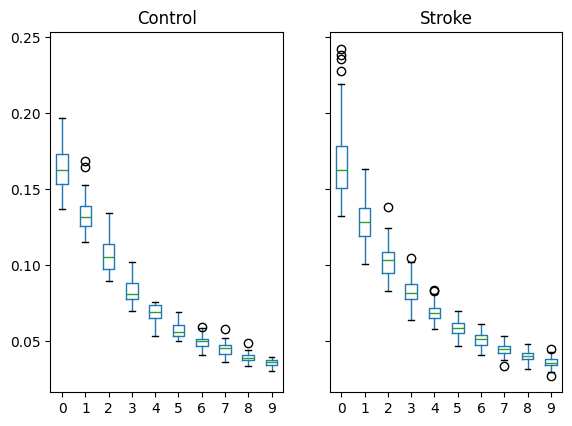
\includegraphics[width=0.5\textwidth]{figures/supp_fig1.png}
\renewcommand{\figurename}{Supplementary Figure}
\caption{\label{fig:lambdas} Scaled eigenvalues of the 10 gradients for control and stroke subjects.  } 
\end{figure}

\begin{figure}[b]
\centering
\includegraphics[width=1\textwidth]{figures/supp_fig2.pdf}
\caption{\label{fig:lags_hist}  Minimum and maximum lag values of control and stroke subjects.}
\end{figure}

\begin{figure}[b]
\centering
\includegraphics[width=1\textwidth]{figures/supp_fig3.pdf}
\caption{\label{fig:1d_edfunc}  Significant regions-wise 1D $\textit{ED}_{{func}}$ differences (p < 0.05 , corrected via permutation
procedure).}
\end{figure}
\end{document}
